% Options for packages loaded elsewhere
\PassOptionsToPackage{unicode}{hyperref}
\PassOptionsToPackage{hyphens}{url}
\PassOptionsToPackage{dvipsnames,svgnames,x11names}{xcolor}
%
\RequirePackage[l2tabu,orthodox]{nag}
\documentclass[%
	12pt,
		oneside,
		letterpaper
]{book}

\usepackage{amsmath,amssymb}
\usepackage{iftex}
\ifPDFTeX
  \usepackage[T1]{fontenc}
  \usepackage[utf8]{inputenc}
  \usepackage{textcomp} % provide euro and other symbols
\else % if luatex or xetex
  \usepackage{unicode-math}
  \defaultfontfeatures{Scale=MatchLowercase}
  \defaultfontfeatures[\rmfamily]{Ligatures=TeX,Scale=1}
\fi
\usepackage{lmodern}
\ifPDFTeX\else  
    % xetex/luatex font selection
\fi
% Use upquote if available, for straight quotes in verbatim environments
\IfFileExists{upquote.sty}{\usepackage{upquote}}{}
\IfFileExists{microtype.sty}{% use microtype if available
  \usepackage[]{microtype}
  \UseMicrotypeSet[protrusion]{basicmath} % disable protrusion for tt fonts
}{}
\usepackage{xcolor}
\setlength{\emergencystretch}{3em} % prevent overfull lines
\setcounter{secnumdepth}{5}


\providecommand{\tightlist}{%
  \setlength{\itemsep}{0pt}\setlength{\parskip}{0pt}}\usepackage{longtable,booktabs,array}
\usepackage{calc} % for calculating minipage widths
% Correct order of tables after \paragraph or \subparagraph
\usepackage{etoolbox}
\makeatletter
\patchcmd\longtable{\par}{\if@noskipsec\mbox{}\fi\par}{}{}
\makeatother
% Allow footnotes in longtable head/foot
\IfFileExists{footnotehyper.sty}{\usepackage{footnotehyper}}{\usepackage{footnote}}
\makesavenoteenv{longtable}
\usepackage{graphicx}
\makeatletter
\newsavebox\pandoc@box
\newcommand*\pandocbounded[1]{% scales image to fit in text height/width
  \sbox\pandoc@box{#1}%
  \Gscale@div\@tempa{\textheight}{\dimexpr\ht\pandoc@box+\dp\pandoc@box\relax}%
  \Gscale@div\@tempb{\linewidth}{\wd\pandoc@box}%
  \ifdim\@tempb\p@<\@tempa\p@\let\@tempa\@tempb\fi% select the smaller of both
  \ifdim\@tempa\p@<\p@\scalebox{\@tempa}{\usebox\pandoc@box}%
  \else\usebox{\pandoc@box}%
  \fi%
}
% Set default figure placement to htbp
\def\fps@figure{htbp}
\makeatother

\directlua{pdf.setminorversion(6)}
% \usepackage[T1]{fontenc}
% \usepackage[utf8]{inputenc}

\usepackage[english]{babel}
\usepackage[otfmath]{XCharter}
\usepackage[strict]{csquotes}

% Change contents title to Table of Contents
\addto\captionsenglish{% Replace "english" with the language you use
  \renewcommand{\contentsname}%
    {Table of contents}%
}

% Bibliography
\usepackage[%
	backend=biber,
	style=ieee, % pick whatever style you want
	sorting=ydnt,
	isbn=true,
]{biblatex}
\addbibresource{bibliography.bib}

% Line spacing
\usepackage{setspace}

\usepackage{etoolbox}

\usepackage[unicode=false]{hyperref}

% \usepackage[notbib,notindex]{tocbibind}

\usepackage[%
	%textwidth=345pt, % Default textwidth
	% marginpar=4cm, % Make marginal notes wider
	% includemp, % Include marginpar in width
	margin=1in,
	left=1.5in, % Left margin must be at least 1.5 inch
]{geometry}

% Toggle for double spaced or not
% \newbool{doublespaced}
\usepackage{titlesec}
   

\titleformat{\part}[display]{\normalfont\large}{Part \ \thepart}{2em}{}[]
\titleformat{\chapter}[block]{\normalfont\Large}{Chapter \ \thechapter:}{1em}{}[]
\titleformat{name=\chapter,numberless}[block]{\normalfont\Large}{}{1em}{\centering}[]
\titleformat{\section}{\normalfont\large}{\thesection}{1em}{}
\titleformat{\subsection}{\normalfont\normalsize}{\thesubsection}{1em}{}
\makeatletter
\@ifpackageloaded{bookmark}{}{\usepackage{bookmark}}
\makeatother
\makeatletter
\@ifpackageloaded{caption}{}{\usepackage{caption}}
\AtBeginDocument{%
\ifdefined\contentsname
  \renewcommand*\contentsname{Table of contents}
\else
  \newcommand\contentsname{Table of contents}
\fi
\ifdefined\listfigurename
  \renewcommand*\listfigurename{List of Figures}
\else
  \newcommand\listfigurename{List of Figures}
\fi
\ifdefined\listtablename
  \renewcommand*\listtablename{List of Tables}
\else
  \newcommand\listtablename{List of Tables}
\fi
\ifdefined\figurename
  \renewcommand*\figurename{Figure}
\else
  \newcommand\figurename{Figure}
\fi
\ifdefined\tablename
  \renewcommand*\tablename{Table}
\else
  \newcommand\tablename{Table}
\fi
}
\@ifpackageloaded{float}{}{\usepackage{float}}
\floatstyle{ruled}
\@ifundefined{c@chapter}{\newfloat{codelisting}{h}{lop}}{\newfloat{codelisting}{h}{lop}[chapter]}
\floatname{codelisting}{Listing}
\newcommand*\listoflistings{\listof{codelisting}{List of Listings}}
\makeatother
\makeatletter
\makeatother
\makeatletter
\@ifpackageloaded{caption}{}{\usepackage{caption}}
\@ifpackageloaded{subcaption}{}{\usepackage{subcaption}}
\makeatother

\usepackage[style=ieee,]{biblatex}
\addbibresource{pubs.bib}
\usepackage{bookmark}

\IfFileExists{xurl.sty}{\usepackage{xurl}}{} % add URL line breaks if available
\urlstyle{same} % disable monospaced font for URLs
\hypersetup{
  pdftitle={Measuring Network Dependencies from Node Activations},
  pdfauthor={Rachael T.B. Sexton},
  colorlinks=true,
  linkcolor={blue},
  filecolor={Maroon},
  citecolor={Blue},
  urlcolor={Blue},
  pdfcreator={LaTeX via pandoc}}


\title{Measuring Network Dependencies from Node Activations}
\author{Rachael T.B. Sexton}
\date{2024-12-31}

\begin{document}

% \frontmatter
\pagestyle{empty}
\singlespacing

%Abstract Page
\hbox{\ }

\begin{center}
\large{{ABSTRACT}}

\vspace{3em}

\end{center}
\hspace{-.15in}
\begin{tabular}{p{0.35\linewidth}p{0.6\linewidth}}
Title of Dissertation:     & {\large \uppercase{Measuring Network
Dependencies from Node Activations}}\\
                           & {\large  Rachael T.B. Sexton } \\
                           & {\large Doctor of Philosophy, } \\
\                         \\
Dissertation Directed by:  & {\large Professor Mark D. Fuge } \\
                           & {\large Department of Mechanical
Engineering} \\
\end{tabular}

\vspace{3em}

% Use word count on the text file
% \begin{doublespacing}

\renewcommand{\baselinestretch}{2}
\large \normalsize
My abstract for this dissertation.\par
% \end{doublespacing}
\clearpage%Titlepage

\thispagestyle{empty} \hbox{\ } \vspace{1.5in}
\renewcommand{\baselinestretch}{1}
\small\normalsize
\begin{center}

\large{\uppercase{Measuring Network Dependencies from Node
Activations}}\\
\ \\ 
\ \\
\large{by} \\
\ \\
\large{Rachael T.B. Sexton}
\ \\
\ \\
\ \\
\ \\
\normalsize
Dissertation submitted to the Faculty of the Graduate School of the \\
University of Maryland, College Park in partial fulfillment \\
of the requirements for the degree of \\
Doctor of Philosophy \\

\end{center}

\vspace{7.5em}

\noindent Advisory Committee: \\
\hbox{\ }\hspace{.5in}Professor Mark D. Fuge, Chair/Advisor \\
\hbox{\ }\hspace{.5in}Professor Jordan L. Boyd-Graber \\
\hbox{\ }\hspace{.5in}Professor Maria K. Cameron \\
\hbox{\ }\hspace{.5in}Professor Michelle Girvan \\
\hbox{\ }\hspace{.5in}Professor Vincent P. Lyzinski \\
 \doublespacing

% \pagestyle{plain} \pagenumbering{roman} \setcounter{page}{2}

% 

% 
% \cleardoublepage

\bookmarksetup{startatroot}

\chapter*{Preface}\label{preface}
\addcontentsline{toc}{chapter}{Preface}

\markboth{Preface}{Preface}

\pagenumbering{roman}

\bookmarksetup{startatroot}

\chapter*{Foreward}\label{foreward}
\addcontentsline{toc}{chapter}{Foreward}

\markboth{Foreward}{Foreward}

\bookmarksetup{startatroot}

\chapter*{Acknowledgements}\label{acknowledgements}
\addcontentsline{toc}{chapter}{Acknowledgements}

\markboth{Acknowledgements}{Acknowledgements}

\addcontentsline{toc}{chapter}{Table of Contents}
    \renewcommand{\contentsname}{Table of Contents}
\renewcommand{\baselinestretch}{1}
\small\normalsize
\tableofcontents %(required, lower-case Roman)
\newpage

\phantomsection %create the correct anchor for the bookmark
\addcontentsline{toc}{chapter}{List of Tables}
    \renewcommand{\contentsname}{List of Tables}
\listoftables %(if present, lower-case Roman)
\newpage

\phantomsection %create the correct anchor for the bookmark
\addcontentsline{toc}{chapter}{List of Figures}
    \renewcommand{\contentsname}{List of Figures}
\listoffigures %(if present, lower-case Roman)
\newpage

% LIST OF ABBREVIATIONS
\phantomsection %create the correct anchor for the bookmark
% \addcontentsline{toc}{chapter}{List of Abbreviations}
% \include{Abbreviations-supertabular}
% TODO use acronym extension??

\newpage
\setlength{\parskip}{0em}
\renewcommand{\baselinestretch}{2}
\small\normalsize

\pagenumbering{arabic}

\bookmarksetup{startatroot}

\chapter{Introduction}\label{introduction}

A wide variety of fields show consistent interest in inferring latent
network structure from observed interactions, from human cognition and
social infection networks, to marketing, traffic, finance, and many
others. \autocite{Inferringnetworksdiffusion_GomezRodriguez2012}
However, an increasing number of authors are noting a lack of agreement
in how to approach the metrology of this problem. This includes rampant
disconnects between the theoretical and methodological network analysis
sub-communities\autocite{Statisticalinferencelinks_Peel2022}, treatment
of error as purely aleatory, rather than epistemic
\autocite{Measurementerrornetwork_Wang2012}, or simply ignoring
measurement error in network reconstruction
entirely\autocite{ReconstructingNetworksUnknown_Peixoto2018}.

Networks in the ``wild'' rarely exist of and by themsleves. Rather, they
are a model of interaction or relation \emph{between} things that were
observed. One of the most beloved examples of a network, the famed
\emph{Zachary's Karate Club}{[}CITE{]}, is in fact reported as a list of
pairwise interactions: every time a club member interacted with another
(outside of the club), Zachary recorded it as two integers (the IDs of
the members). The final list of pairs can be \emph{interpreted} as an
``edge list'', which can be modeled with a network: a simple graph. This
was famously used to show natural community structure that nicely
matches the group separation that eventually took place when the club
split into two.{[}CITE{]}

Note, however, that we could have just as easily taken note of the
instigating student for each interaction (i.e.~which student initiated
conversation, or invited the other to socialize, etc.). If that
relational asymmetry is available, our ``edges'' are now
\emph{directed}, and we might be able to ask questions about the rates
that certain students are asked vs.~do the asking, and what that implies
about group cohesion. Additionally, the time span is assumed to be ``for
the duration of observation'' (did the students \emph{ever} interact),
but if observation time was significantly longer, say, multiple years,
we might question the credulity of treating a social interaction 2 years
ago as equally important to an interaction immediately preceding the
split. This is now a ``dynamic'' graph; or, if we only measure relative
to the time of separation, at the very least a ``weighted'' one.

\emph{We do not know if any of these are true}. In fact, do to ambiguous
reporting in the original work, we do not know if the network being
described from the original edge data even has 77 or 78 edges. Lacking a
precise definition of what the graph's components (i.e.~it's edges) are,
\emph{as measurable entities}, means we cannot estimate the measurement
error in the graph.

To begin adressing these issues, this introductory section returns to
foundational statistical measurment concepts and terminology, while
clarifying each concepts potential relationships to the problems of
network structure metrology.\\
First, what ``measurement'' means in this context, and specifically the
ways we encode observations, operations, and uncertainties numerically.
Second, what ``relation'' means, since network structure is intended to
encode such relations as a mathematical object, despite common
ambiguities and confusion around what practitioners intend on
communicating through them.

{[}FUTURE SECTIONS?{]}

\part{A Practitioner's Guide to Network Recovery}

\chapter{Metrology as matrices}\label{metrology-as-matrices}

Where metrology is concerned, the actual unit of observation and how it
is encoded for us is critical to how analysts may proceed with
quantifying, modeling, and measuring uncertainty around observed
phenomena. Experiment and observation tends to be organized as inputs
and outputs, or, independent variables and dependent variables,
specifically. Independent variables are observed, multiple times
(``observations''), and changes in outcome for each can be compared to
the varying values associated with the independent variable input
(``features''). For generality, say a practitioner records their
measurements as scalar values,
i.e.~\(x\in\mathbb{S}\in\{\mathbb{R,Z,N},\cdots\}\). The structure most
often used to record scalar values of \(n\) independent/input variable
features over the course of \(m\) observations is called a design matrix
\(X:\mathbb{S}^{m\times n}\).\footnote{ Not all observations are scalar,
  but they can become so. If individual measurments are
  higher-dimensional (e.g.~images are 2D), X is a tensor, which can be
  transformed through unrolling or embedding into a lower dimensional
  representation before proceeding. There are other techniques for
  dealing with e.g.~categorical data, such as one-hot encoding (where
  the features are binary for each possible category, with boolean
  entries for each observation).}

\section{Observation and feature
``spaces''}\label{observation-and-feature-spaces}

If we index a set of observations and features, respectively, as
\[ i\in I=\{1,\cdots,m\}, \quad j\in J=\{1,\cdots,n\},\qquad I,J:\mathbb{N}\]
then the design matrix can map the index of an observation and a feature
to the corresponding measurement.
\[x=X(i,j)\qquad X : I\times J \rightarrow \mathbb{S}\] i.e.~the
measured value of the \(j\)th independent variable from the \(i\)th
observation. In this scheme, an ``observation'' is a single row vector
of features in \(\mathbb{S}^{n\times 1}\) (or simply
\(\mathbb{S}^{n}\)), such that each observation encodes a position in
the space defined by the features, i.e.~the \emph{feature space}, and
extracting a specific observation vector \(i\) from the entire matrix
can be denoted as
\[\mathbf{x}_i=X(i,\cdot),\quad \mathbf{x}:J\rightarrow\mathbb{S}\]
Similarly, every ``feature'' is associated with a single column vector
in \(\mathbb{S}^{1\times m}\), which can likewise be interpreted as a
position in the space of observations (the \emph{data space}):
\[\mathbf{x}_j^*=X(\cdot,j),\quad \mathbf{x}^*:I\rightarrow\mathbb{S}\]
Note that this definition could be swapped without loss of generality.
In other words, \(\mathbf{x}\) and \(\mathbf{x}^*\) being in row and
column spaces is somewhat arbitrary, having more to do with the
logistics of experiment design and data collection. We could have
measured our feature vectors one-at-a-time, measuring their values over
an entire ``population'', in effect treating that as the independent
variable set.\footnote{ In fact, vectors are often said to be in the
  column-space of a matrix, especially when using them as
  transformations in physics or deep learning layers. We generally
  follow a one-observation-per-row rule, unless otherwise stated.}

To illustrate this formalism in a relevant domain, let's take another
classic network example from academia: co-citation networks. {[}DRAW
BIPARTITE{]} Lists of co-authors on publications is often reported as
``network'' data, and subjected to network analysis techniques. For
\(m\) papers we might be aware of a total of \(n\) authors. For a given
paper, we are able to see which authors are involved, and we say those
authors ``activated'' for that paper. It makes sense that our
observations are individual papers, while the features might be the set
of possible authors. However, we are not given information about which
author was invited by which other one, or when each author signed on. In
other words, the measured values are strictly boolean, and we can
structure our dataset as a design matrix \(X:\mathbb{B}^{m\times n}\).
We can then think of the \(i^{\mathrm{th}}\) paper as being represented
by a vector \(\mathbf{x}_i:\mathbb{B}^n\), and proceed using it in our
various statistical models. If we desired to analyze the set of authors,
say, in order to determine their relative neighborhoods or latent author
communities, we could equally use the feature vectors for each paper,
this time represented in a vector
\(\mathbf{x}^*_j:\mathbb{B}^{1\times m}\).

\section{Models \& linear operators}\label{models-linear-operators}

Another powerful tool an analyst has is \emph{modeling} the observation
process. This is relevant when the observed data is hypothesized to be
generated by a process we can represent mathematically, but we do not
know the parameter values to best represent the observations (or the
observations are ``noisy'' and we want to find a ``best'' parameters
that account for this noise). This is applicable to much of scientific
inquiry, though one common use-case is the de-blurring of observed
images (or de-noising of signals), since we might have a model for how
blurring ``operated'' on the original image to give us the blurred one.
We call this ``blurring'' a \emph{linear operator} if it can be
represented as a matrix\footnote{in the finite-dimensional case}, and
applying it to a model with \(l\) parameters is called the \emph{forward
map}:
\[\mathbf{x} = F\mathbf{p}\qquad F:\mathbb{R}^{l}\rightarrow \mathbb{R}^n\]
where \(P\) is the space of possible parameter vectors, i.e.~the
\emph{model space}. The forward map takes a modeled vector and predicts
a location in data space.

Of critical importance, then, is our ability to recover some model
parameters from our observed data, e.g.~if our images were blurred
through convolution with a blurring kernel, then we are interested in
\emph{deconvolution}. If \(F\) is invertible, the most direct solution
might be to apply the operator to the data, as the \emph{adjoint map}:
\[ \mathbf{p} = F^H\mathbf{x}\qquad F^H:\mathbb{R}^{n}\rightarrow \mathbb{R}^l\]
which removes the effect of \(F\) from the data \(\mathbf{x}\) to
recover the desired model \(\mathbf{p}\).

Trivially we might have an orthogonal matrix \(F\), so \(F^H=F^{-1}\) is
available directly. In practice, other approaches are used to minimize
the \emph{residual}:
\(\hat{\mathbf{p}}^=\min_{\mathbf{p}} F\mathbf{p}-\mathbf{x}\). Setting
the gradient to 0 yeilds the normal equation, such that
\[ \hat{\mathbf{p}}=(F^TF)^{-1}F^T\mathbf{x}\] This should be familiar
to readers as equivalent to solving ordinary least-squares (OLS).
However, in that case it is more often shown as having the \emph{design
matrix} \(X\) in place of the operator \(F\).

\emph{This is a critical distinction to make:} OLS as a ``supervised''
learning method treats some of the observed data we represented as a
design matrix previously as a target to be modeled, \(y=X(\cdot,j)\),
and the rest maps parameters into data space, \(F=X(\cdot,J/j)\). With
this paradigm, only the target is being ``modeled'' and the rest of the
data is used to create the operator. In the citation network example, it
would be equivalent to trying to predict one author's participation in
every paper, \emph{given} every other author's participation in them.

For simplicity, most work in the supervised setting treats the reduced
data matrix as X, opting to treat \(y\) as a separate \emph{dependent
variable}. However, our setting will remain \emph{unsupervised}, since
no single target variable is of specific interest---all observations are
``data''. In this, we more closely align with the deconvolution
literature, such that we are seeking a model and an operation on it that
will produce the observed behavior in an ``optimal'' way.

\section{Measurement quantification \&
error}\label{measurement-quantification-error}

\begin{itemize}
\tightlist
\item
  marginal sums
\item
  rule of succession
\item
  type I and II Error?
\item
  Epistemic and Alleatoric Uncertainty?
\end{itemize}

Ultimately we are not great at specifying what ``being related''
actually means\ldots{}

\section{Incidence vs.~Proximity}\label{incidence-vs.-proximity}

\subsection{Incidence structures \&
dependency}\label{incidence-structures-dependency}

foundational model of graph theory and incidence structures more
broadly. More to come, but get the terminology down.

Spring example, road example, etc. Discuss Complex Systems and their
representation.

\subsection{Kernels \& distances}\label{kernels-distances}

Importantly for the use of linear algebra, these values assigned for
each feature are assumed to exist in a field (or, more generally, a
semiring) \(R\), equipped with operators analogous to addition
(\(\oplus\)) and multiplication (\(\otimes\)) that allow for values to
be aggregated through an inner product. The matrix of all pairs of
inner-products found by matrix multiplication (contracting over the
feature space) is given by:

\[G(\mathbf{x}_i, \mathbf{x}_j,R) = G_{ij} = \bigoplus_{k=1}^{n} x_{ik} \otimes x_{kj} \]

such that real-valued entries and a traditional ``plus-times'' inner
product recovers the Gram matrix \(G_{ij}=\sum_{k=1}^{n} x_{ik}x_{kj}\),
or simply \(G=X^TX\).

How ``close'' or ``far away'' things are\ldots. Avrachenkov et al.~

Important: these measurements often assume distance is defined in terms
of the measurements/objects/data, but for \emph{inverse problems},
structure learning, etc., they are more often applied in terms of the
features/operators.

Example with doc-term matrices

The inner product between two papers will yield a ``true'' only if two
papers share at least one author in common. This is called a
\emph{bipartite projection}{[}CITE{]}, specifically the ``papers''
projection.

Similarly, if our goal is to determine a network of ``whether two
authors ever coauthored'', we could perform a bipartite projection using
the boolean inner product in the observation space i.e.~the ``authors''
projection. It is this second projection, for determining a structure
between features embedded into the ``observation'' space, that we are
primarily concerned with in this work, since it is the view that most
closely resembles the concept of covariance or correlation between
independent variables (features) in statistics more generally.

\subsection{Implications for networks}\label{implications-for-networks}

Usually dependencies are taken as causing or enabling proximity. E.g.
shortest paths, vs.~edges.

The approach taken by researchers/investigators\ldots do they assume a
level of interchangeability between the two kinds of ``relation''? Do
they define Or do they

\chapter{Incidence in Vector Space}\label{incidence-in-vector-space}

From \autocite{WhyHowWhen_Torres2021}, and linalg book, and hypergraph
incidence model

For each, describe the meaning of

\begin{enumerate}
\def\labelenumi{\arabic{enumi}.}
\tightlist
\item
  Observation model (and connection to node activation data)
\item
  Vector space representation
\item
  Inner product (linear kernel)
\item
  Induced Norms
\end{enumerate}

\section{Graphs}\label{graphs}

Initial notation (set-based) and outline of section

\begin{figure}[H]

{\centering \pandocbounded{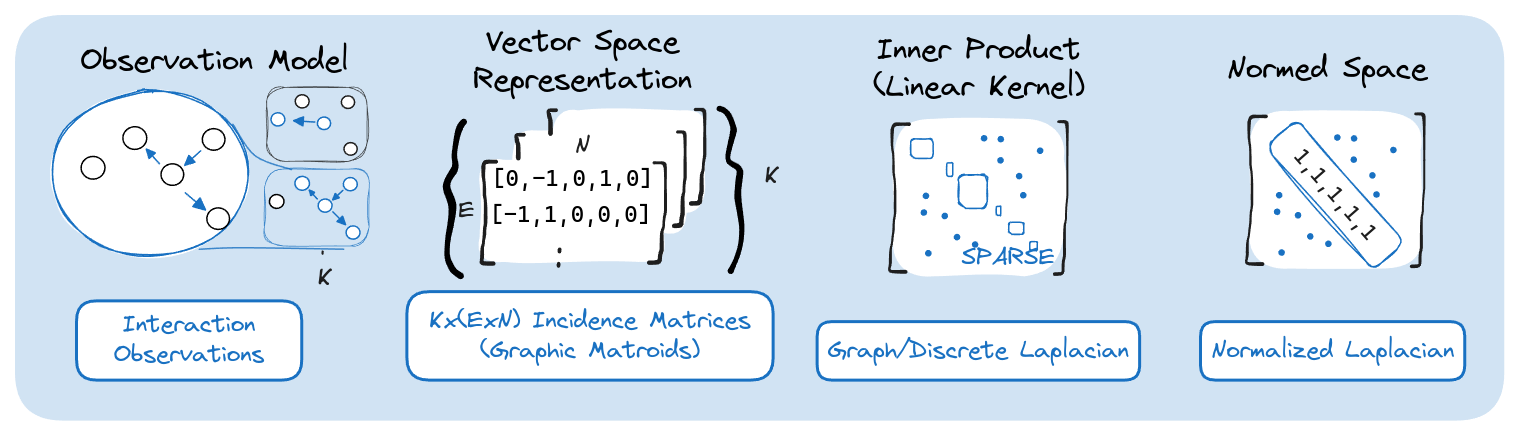
\includegraphics[keepaspectratio]{images/relation-observations.png}}

}

\caption{Edge Relation Observational Model}

\end{figure}%

\subsection{Edges as Vectors of Nodes}\label{edges-as-vectors-of-nodes}

\subsection{Inner Product on Edges}\label{inner-product-on-edges}

Laplacian as inner product on incidence observations. Associated objects
(degree vector, o)

Rescaling to achieve normaalization.

Use to define kernels (and application e.g.~soft-cosine measure)

\subsection{From Edge Observations to Node
Activations}\label{from-edge-observations-to-node-activations}

Strictly speaking, we can't say that nodes are directly observed in this
space\ldots{} edges are. Collections of nodes are measured two-at-a-time
(one-per-edge being traversed).

Another way to approach is to view inner products as a sum of outer
products. A each edge uniquely corresponds to 2 nodes (in a simple
graph). Use triangle unfolding for closed form bijection.

Unrolling 3D tensor of subgraphs along eads to a secondary
representation of graphs as an \emph{edgelist}, having binary activation
vectors on edges rather than nodes. Then each observation in this model
is necessarily a set of activated edges. The non-zero (visited) nodes
are found using the incidence matrix as an operator.

\section{Hypergraphs}\label{hypergraphs}

\begin{figure}[H]

{\centering \pandocbounded{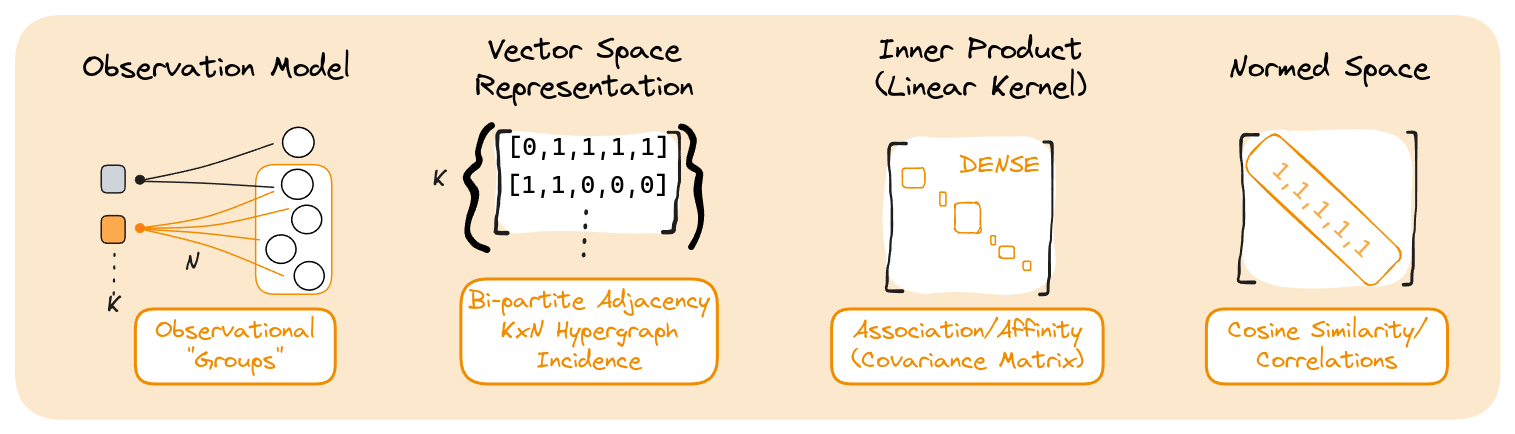
\includegraphics[keepaspectratio]{images/hypergraph-observations.png}}

}

\caption{Hyperedge Relation Observational Model}

\end{figure}%

\subsection{Hyperedges as Vectors of
Nodes}\label{hyperedges-as-vectors-of-nodes}

\subsection{Inner product on
Hyperedges}\label{inner-product-on-hyperedges}

Roundabout way of describing binary/occurrence data. Inner product is
co-occurrences.

Leads to correlation/covariance, etc.

\chapter{Roads to Network Recovery}\label{roads-to-network-recovery}

\section{Choosing a structure recovery
method}\label{choosing-a-structure-recovery-method}

\begin{quote}
Takeaway: a way to organize existing algorithms, AND highlight unique
set of problems we set out to solve
\end{quote}

\section{Organizing Recovery Methods}\label{organizing-recovery-methods}

i.e.~Network Recovery as an Inverse Problem, and what information is had
at each point.

\begin{figure}[H]

{\centering \pandocbounded{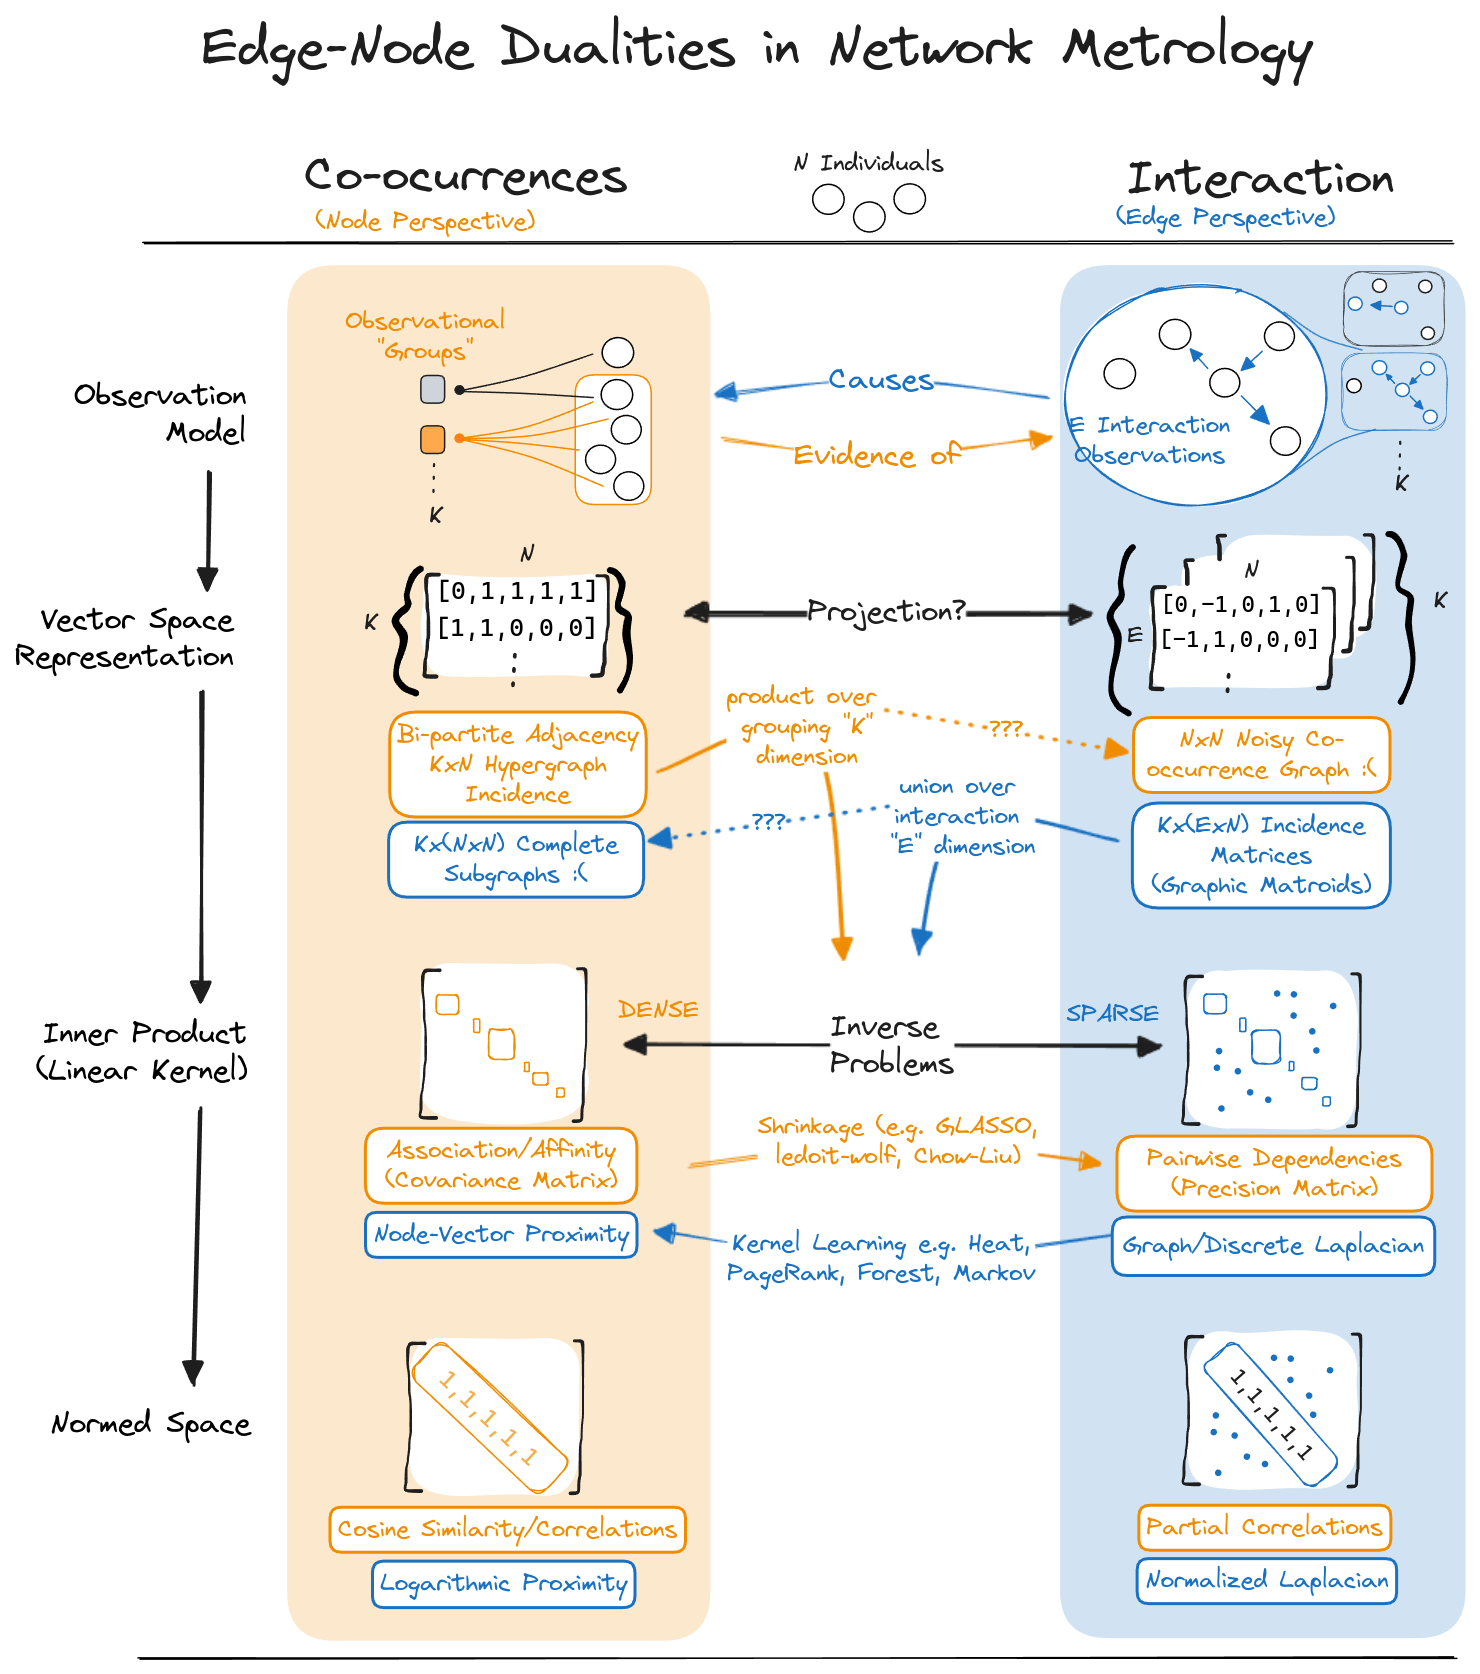
\includegraphics[keepaspectratio]{images/adjoint-cheatsheet.png}}

}

\caption{Relating Graphs and Hypergraph/bipartite structures as adjoint
operators}

\end{figure}%

\subsection{Observing Nodes vs Edges}\label{observing-nodes-vs-edges}

\subsection{Embeddings, Inner Products, \&
Preprocessing}\label{embeddings-inner-products-preprocessing}

\section{Tracing Information Loss
Paths}\label{tracing-information-loss-paths}

\subsection{Table of Existing
Approaches}\label{table-of-existing-approaches}

\begin{itemize}
\tightlist
\item
  Observation-level loss (starting with the inner product or kernel)
\item
  Non-generative model loss (no projection of data into model space)
\item
  no uncertainty quantification
\end{itemize}

\subsection{A Path Forward}\label{a-path-forward}

Sorting algorithms\ldots{} \emph{none address all three!}

i.e.~MOTIVATES FOREST PURSUIT

\part{Nonparametric Network Recovery With Random Spanning Forests}

\texttt{\#\ Recovery\ from\ Bipartite\ Occurrence\ Records}

\begin{itemize}
\tightlist
\item
  A generative model for multi-output binary observations under
  diffusion
\item
  Edge Recovery through Sparse Approximation by Empirical Bayes
\item
  Gibbs Sampling a hierarchical bayesian model
\end{itemize}

\chapter{Random Spanning Forests}\label{random-spanning-forests}

\section{Node Activation by Diffusive
Processes}\label{node-activation-by-diffusive-processes}

Random walks are regularly employed to model spreading and diffusive
processes on networks. If a network consists of locations, states,
agents, etc. as ``nodes'', and relationships between nodes as ``edges'',
then random walks consist of a stochastic process that ``visits'' nodes
by randomly ``walking'' between them along connecting edges.
Epidemiological models, cognitive search in semantic networks, stock
price influences, website traffic routing, social and information
cascades, and many other domains also involving complex systems, have
used the statistical framework of random walks to describe, alter, and
predict their behaviors. If a network structure is known ahead of time,
the dynamics of random-walks might be used to capture the network
structure via sampling, estimate node importance's, or predict
phase-changes in node states (e.g.~infected vs.~uninfected)

In many cases, however, the existence of relationships is not known
already, and analysts might \emph{assume} their data was generated by
random-walk-like processes, and want to use that knowledge to estimate
the underlying structure of the relationships between nodes.

\subsection{Dependencies as Trees}\label{dependencies-as-trees}

\subsection{Matrix-Forest Theorem}\label{matrix-forest-theorem}

\section{Generative Model
Specification}\label{generative-model-specification}

\pandocbounded{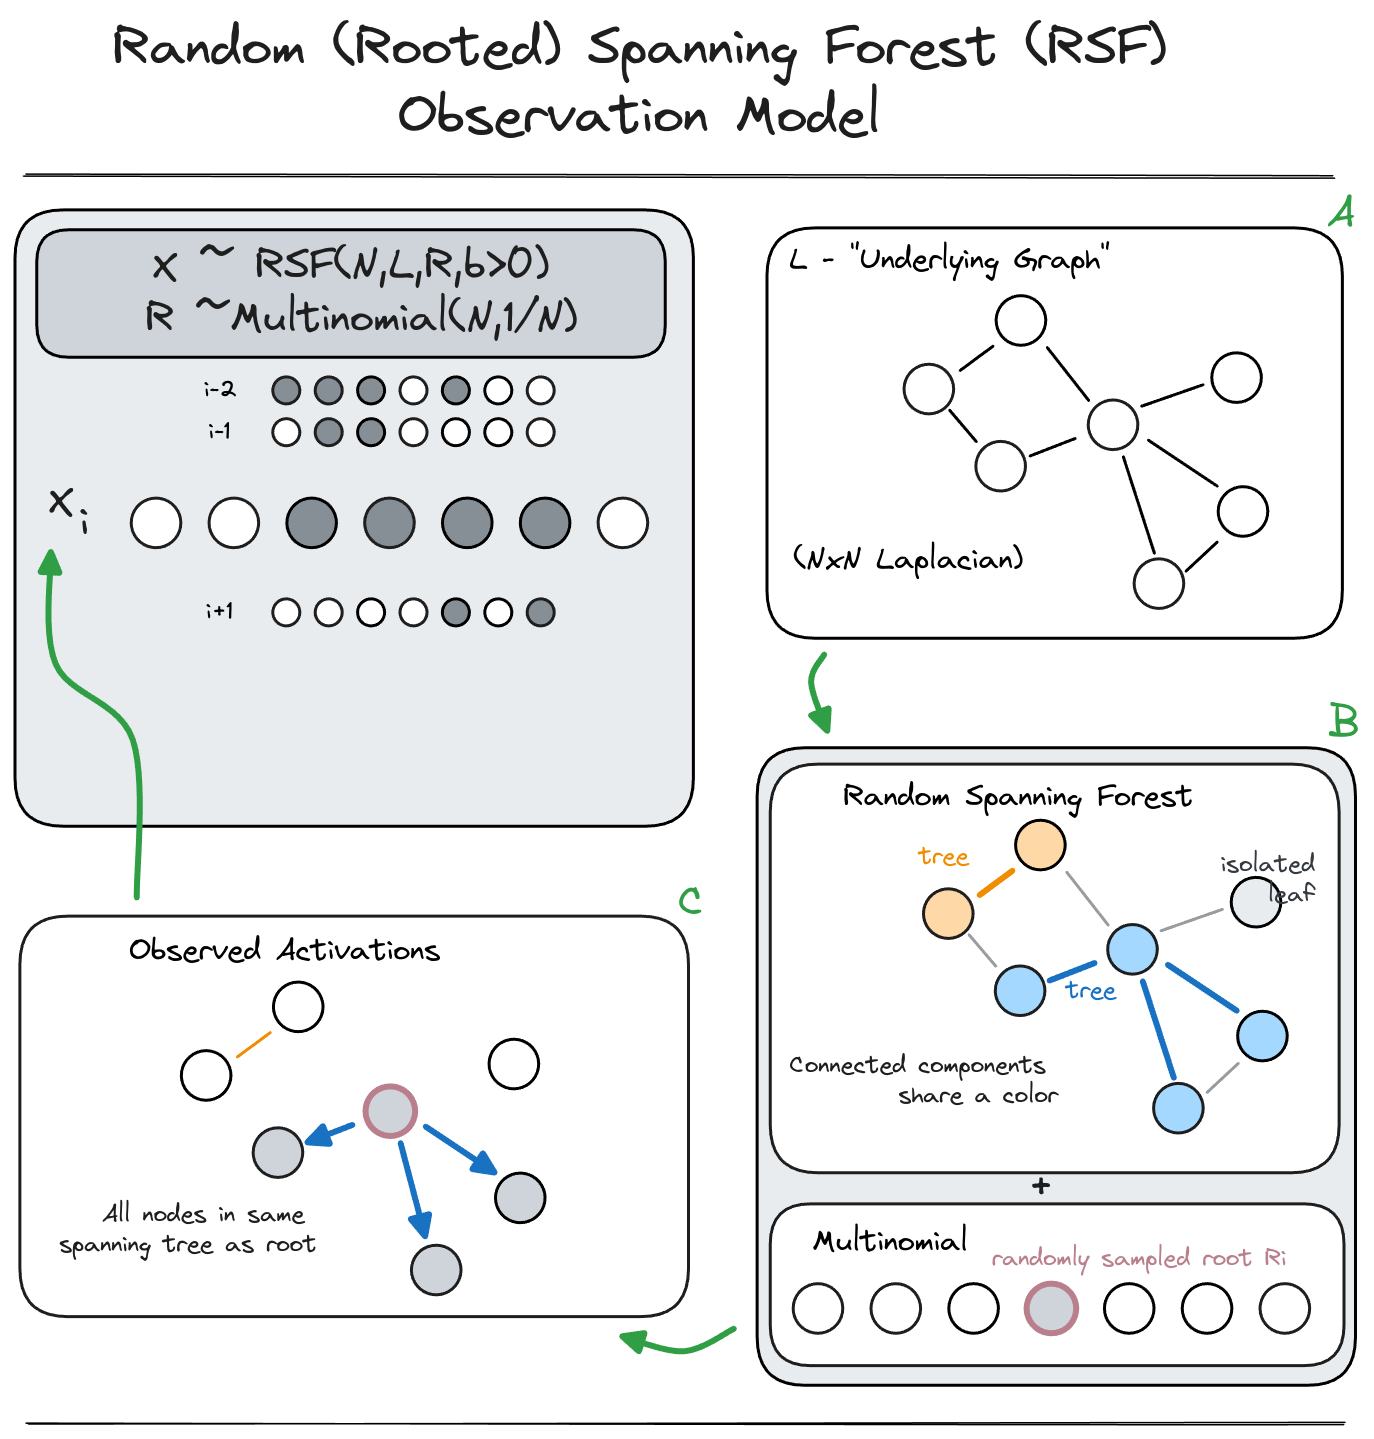
\includegraphics[keepaspectratio]{images/random-spanning-forests.png}}
- hierarchical model - marginalize over the root node.

\chapter{Forest Pursuit: Approximate Recovery in Near-linear
Time}\label{forest-pursuit-approximate-recovery-in-near-linear-time}

\begin{quote}
filling the gap we saw in the literature
\end{quote}

\section{Sparse Dictionary Learning}\label{sparse-dictionary-learning}

\subsection{Problem Speification}\label{problem-speification}

\subsection{Matching Pursuit}\label{matching-pursuit}

\subsection{Space of Spanning Forests}\label{space-of-spanning-forests}

\section{Forest Pursuit: Approximate Recovery in Near-linear
Time}\label{forest-pursuit-approximate-recovery-in-near-linear-time-1}

I.e. the PLOS paper (modified basis-pursuit via MSTs) \#\#\# Algorithm
Summary

\subsection{Uncertainty Estimation}\label{uncertainty-estimation}

\subsection{Approximate Complexity}\label{approximate-complexity}

\section{Simulation Study}\label{simulation-study}

\subsection{Method}\label{method}

\subsection{Results}\label{results}

\subsection{Discussion}\label{discussion}

\chapter{LFA: Latent Forest
Allocation}\label{lfa-latent-forest-allocation}

\section{Radom Spanning Trees}\label{radom-spanning-trees}

\begin{itemize}
\tightlist
\item
  Methods for sampling i.e.~wilson's and Duan's (other? Energy paper?)
\item
  Tree Likelihoods, other facts
\end{itemize}

\section{Bayesian Estimation by Gibbs
Sampling}\label{bayesian-estimation-by-gibbs-sampling}

\begin{itemize}
\tightlist
\item
  comparison with LDA
\item
  Simplifying Assumptions (conditional prob IS prob for this)
\end{itemize}

I.e. the unwritten paper, modifying technique by
\textcite{BayesianSpanningTree_Duan2021} for RSF instead of RSTs

\section{Simulation Study}\label{simulation-study-1}

Kind of unsure here.

\part{Application and Future Development}

\chapter{Qualitative Application of Relationship
Recovery}\label{qualitative-application-of-relationship-recovery}

\chapter{Recovery from Ordered Random-Walk Observation
Sets}\label{recovery-from-ordered-random-walk-observation-sets}

Like before, but with the added twist of \emph{knowing} our nodes were
activated with a particular partial order.

\emph{insert from
\autocite{OrganizingTaggedKnowledge_Sexton2020,UsingSemanticFluency_Sexton2019}}


\printbibliography



\end{document}
